% SABD Project 2 — oral presentation
% Beamer, Boadilla theme. Compile with pdfLaTeX in Overleaf.
\documentclass[aspectratio=169,10pt]{beamer}

% ------ theme & colours -----------------------------------------------------
\usetheme{Boadilla}
\usecolortheme{seahorse}
\setbeamertemplate{navigation symbols}{}
\setbeamertemplate{footline}[frame number]

\usepackage[utf8]{inputenc}
\usepackage[T1]{fontenc}
\usepackage{xcolor}
\usepackage{booktabs}
\usepackage{tikz}
\usepackage{array}
\usepackage{colortbl}
\usetikzlibrary{arrows.meta,positioning}

\definecolor{sabdNavy}{HTML}{1E2761}
\definecolor{sabdIce}{HTML}{CADCFC}
\definecolor{sabdOrange}{HTML}{D86F0E}
\definecolor{sabdGreen}{HTML}{2E7D32}
\definecolor{sabdRed}{HTML}{C62828}
\definecolor{sabdGrey}{HTML}{555555}
\definecolor{sabdLight}{HTML}{F4F6FC}

% Re-skin headers/structure in navy
\setbeamercolor{structure}{fg=sabdNavy}
\setbeamercolor{frametitle}{fg=sabdNavy}
\setbeamercolor{title}{fg=sabdNavy}
\setbeamercolor{subtitle}{fg=sabdGrey}
\setbeamerfont{frametitle}{series=\bfseries,size=\Large}

% ------ metadata ------------------------------------------------------------
\title[SABD Project 2]{Real-Time Analysis of US Flight Delays\\ with Apache Flink}
\subtitle{Event-Time Windowing, Stream Simulation,\\
  and a Hybrid Stream/Batch Fallback for Top-K Ranking}
\author[Daniel Garoz]{Daniel Garoz}
\institute[Tor Vergata]{Universit\`a degli Studi di Roma Tor Vergata \\
  SABD Project 2 \textbar{} A.A.\ 2025/26}
\date{}

\begin{document}

% ============================================================================
\begin{frame}[plain]
  \titlepage
\end{frame}

% ============================================================================
\begin{frame}{Project goals}
\textbf{Single-student team — Q1 and Q2 mandatory (Q3 skipped).}
\vspace{0.5em}

\begin{columns}[T,onlytextwidth]
\column{0.48\textwidth}
{\color{sabdNavy}\textbf{Q1 — Hourly carrier statistics}}
\begin{itemize}\small
  \item Carriers AA, DL, UA, WN
  \item Tumbling event-time windows of 1\,h
  \item Per (window, carrier): total, completed, cancelled, diverted
  \item Mean \texttt{DEP\_DELAY} (non-cancelled)
  \item Cancellation rate, late-departure rate
\end{itemize}

\column{0.48\textwidth}
{\color{sabdOrange}\textbf{Q2 — Top-10 airports, severe delays}}
\begin{itemize}\small
  \item All carriers, by \texttt{ORIGIN\_AIRPORT\_ID}
  \item Severe = valid \& \texttt{DEP\_DELAY} $>$ 30\,min
  \item Three windows: 1\,h, 6\,h, full dataset
  \item Filter: $\geq 30$ valid flights / airport
  \item Top-10 by severe-count, plus top-20 delayed list
\end{itemize}
\end{columns}

\vspace{1em}
\centerline{\footnotesize\textbf{Dataset:} US BTS, 2{,}229{,}453 flight events, 1\,Jan – 30\,Apr 2025.}
\end{frame}

% ============================================================================
\begin{frame}{System architecture}
\centering
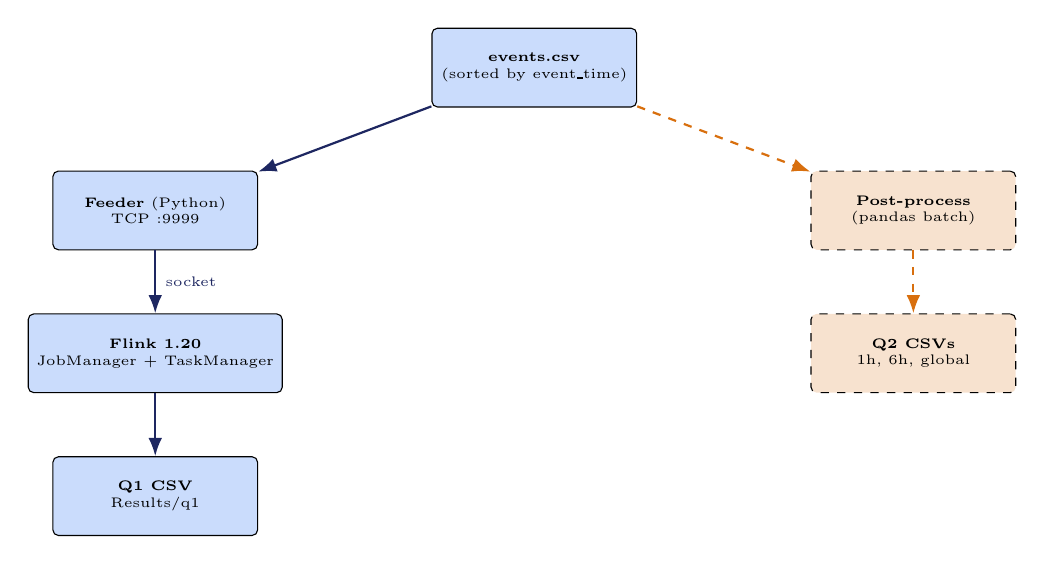
\begin{tikzpicture}[
  every node/.style={align=center, font=\tiny},
  box/.style={draw, rounded corners=2pt, minimum width=26mm, minimum height=10mm, fill=sabdIce, inner sep=3pt},
  side/.style={draw, dashed, rounded corners=2pt, minimum width=26mm, minimum height=10mm, fill=sabdOrange!20, inner sep=3pt},
  pipe/.style={-Latex, thick, sabdNavy},
  dpipe/.style={-Latex, thick, dashed, sabdOrange},
  node distance=8mm and 22mm,
]
  \node[box] (csv) {\textbf{events.csv}\\(sorted by event\_time)};
  \node[box, below left=of csv] (feeder) {\textbf{Feeder} (Python)\\TCP :9999};
  \node[box, below=of feeder] (flink) {\textbf{Flink 1.20}\\JobManager + TaskManager};
  \node[box, below=of flink] (q1) {\textbf{Q1 CSV}\\Results/q1};
  \node[side, below right=of csv] (post) {\textbf{Post-process}\\(pandas batch)};
  \node[side, below=of post] (q2) {\textbf{Q2 CSVs}\\1h, 6h, global};

  \draw[pipe] (csv) -- (feeder);
  \draw[pipe] (feeder) -- node[right, font=\tiny]{socket} (flink);
  \draw[pipe] (flink) -- (q1);
  \draw[dpipe] (csv) -- (post);
  \draw[dpipe] (post) -- (q2);
\end{tikzpicture}

\vspace{0.4em}
\footnotesize
{\color{sabdNavy}\textbf{Solid:} streaming path (Q1)} \quad
{\color{sabdOrange}\textbf{Dashed:} batch path (Q2)}

\medskip
\small 3 Docker containers, bind-mounted project tree, custom Flink image with PyFlink in a venv.
\end{frame}

% ============================================================================
\begin{frame}{Stream simulation}
\begin{columns}[T,onlytextwidth]
\column{0.32\textwidth}
{\color{sabdNavy}\textbf{1. Pre-sort}}
\begin{itemize}\footnotesize
  \item Read 4 monthly CSVs
  \item Build \texttt{event\_time} from year, month, day + \texttt{CRS\_DEP\_TIME}
  \item Sort $\to$ \texttt{events.csv}
  \item No out-of-order at source
\end{itemize}

\column{0.32\textwidth}
{\color{sabdNavy}\textbf{2. Feeder + acceleration}}
\begin{itemize}\footnotesize
  \item TCP server, port 9999
  \item Sleep $\Delta t_{\text{wall}} = (et_{n+1}-et_n)/\alpha$
  \item $\alpha = 60{,}000$ $\to$ 120\,d in $\sim$3\,min
  \item $\alpha$ only compresses wall-clock
  \item Event-time semantics invariant
\end{itemize}

\column{0.32\textwidth}
{\color{sabdNavy}\textbf{3. Watermarking}}
\begin{itemize}\footnotesize
  \item \texttt{bounded\_out\_of\_orderness(60s)}
  \item Defensive jitter buffer
  \item $60\,\text{s} \ll 1\,\text{h}$ smallest window
  \item Null delays $\to$ 0 (spec-permitted)
\end{itemize}
\end{columns}
\end{frame}

% ============================================================================
\begin{frame}{Query 1 — DataStream pipeline}
\begin{columns}[T,onlytextwidth]
\column{0.55\textwidth}
\centering
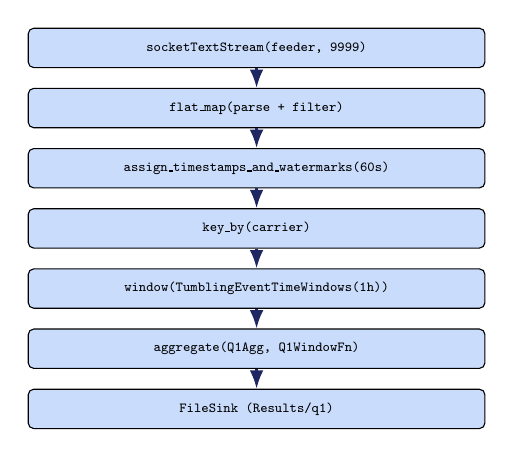
\begin{tikzpicture}[
  every node/.style={align=center, font=\tiny\ttfamily, fill=sabdIce, draw, rounded corners=2pt, minimum width=58mm, minimum height=5mm, inner sep=2pt},
  pipe/.style={-Latex, thick, sabdNavy},
  node distance=2.5mm,
]
  \node (a) {socketTextStream(feeder, 9999)};
  \node[below=of a] (b) {flat\_map(parse + filter)};
  \node[below=of b] (c) {assign\_timestamps\_and\_watermarks(60s)};
  \node[below=of c] (d) {key\_by(carrier)};
  \node[below=of d] (e) {window(TumblingEventTimeWindows(1h))};
  \node[below=of e] (f) {aggregate(Q1Agg, Q1WindowFn)};
  \node[below=of f] (g) {FileSink (Results/q1)};
  \foreach \x/\y in {a/b,b/c,c/d,d/e,e/f,f/g}\draw[pipe] (\x) -- (\y);
\end{tikzpicture}

\column{0.42\textwidth}
{\color{sabdNavy}\textbf{Aggregator state} (7 primitives)}\\[2pt]
\texttt{\scriptsize (num, completed, cancelled,\\
\hphantom{(}diverted, sum\_dep\_delay,\\
\hphantom{(}count\_non\_cancelled,\\
\hphantom{(}late\_non\_cancelled)}
\vspace{1em}

{\color{sabdNavy}\textbf{Window function output}}
\begin{itemize}\footnotesize\setlength\itemsep{2pt}
  \item \texttt{mean = sum / count\_nc}
  \item \texttt{canc\_rate = 100·canc / num}
  \item \texttt{late\_rate = 100·late\_nc / count\_nc}
  \item One CSV line per (window, carrier)
  \item Sustained $\sim$10{,}000\,ev/s
\end{itemize}
\end{columns}
\end{frame}

% ============================================================================
\begin{frame}{Query 1 — Output sample}
\centering\footnotesize
\begin{tabular}{ccccccccrrr}
\toprule
\textbf{start} & \textbf{end} & \textbf{air} & \textbf{num} & \textbf{compl} & \textbf{canc} & \textbf{div} & \textbf{mean} & \textbf{canc\%} & \textbf{late\%} \\
\midrule
01-01 00:00 & 01:00 & AA & 13  & 13  & 0 & 0 & 7.38  & 0.00 & 30.77 \\
01-01 00:00 & 01:00 & DL & 1   & 1   & 0 & 0 & -6.00 & 0.00 & 0.00  \\
01-01 00:00 & 01:00 & UA & 7   & 7   & 0 & 0 & 10.57 & 0.00 & 14.29 \\
04-20 08:00 & 09:00 & AA & 215 & 213 & 2 & 0 & 7.52  & 0.93 & 18.31 \\
04-20 08:00 & 09:00 & DL & 251 & 251 & 0 & 0 & 1.06  & 0.00 & 8.37  \\
04-20 08:00 & 09:00 & WN & 233 & 232 & 1 & 0 & -1.03 & 0.43 & 5.60  \\
\bottomrule
\end{tabular}

\vspace{1em}
{\color{sabdNavy}\textbf{Sanity check}}
\begin{itemize}\footnotesize
  \item \textbf{9{,}765} (window, carrier) rows over 120 days of event time
  \item AA at 04-20 8:00: 215 flights, 2 cancelled (0.93\%), mean delay 7.52\,min, 18.31\% late
  \item Time-of-day pattern matches expected BTS behaviour (low pre-dawn, peak mid-morning)
\end{itemize}
\end{frame}

% ============================================================================
\begin{frame}{Query 2 — Four PyFlink iterations}
\footnotesize
\begin{columns}[T,onlytextwidth]
\column{0.48\textwidth}
{\color{sabdRed}\textbf{v1 — ProcessAllWindowFunction}}
\begin{itemize}\setlength\itemsep{1pt}
  \item \texttt{window\_all} + top-10 in Python
  \item \textbf{OOM at $\sim$900K events}
  \item Beam worker heap ($\sim$134\,MB) exhausted by global 120-day window
\end{itemize}
\vspace{0.4em}

{\color{sabdOrange}\textbf{v3 — v2 + parallelism = 4}}
\begin{itemize}\setlength\itemsep{1pt}
  \item Same as v2 with \texttt{-p 4}
  \item Throughput \textbf{regressed} to $\sim$300\,ev/s
  \item Socket source: parallelism = 1
  \item Beam coordination adds overhead
\end{itemize}

\column{0.48\textwidth}
{\color{sabdOrange}\textbf{v2 — keyBy + PICKLED accumulator}}
\begin{itemize}\setlength\itemsep{1pt}
  \item Pre-aggregation by airport
  \item Acc: (num, severe, sum, max, top20)
  \item \texttt{Types.PICKLED\_BYTE\_ARRAY()}
  \item $\sim$500\,ev/s, 2–3 orders worse than Q1
\end{itemize}
\vspace{0.4em}

{\color{sabdOrange}\textbf{v4 — primitive acc + bundle tuning}}
\begin{itemize}\setlength\itemsep{1pt}
  \item \texttt{Types.TUPLE([INT, INT, DOUBLE, DOUBLE])}
  \item \texttt{bundle.size = 10{,}000}
  \item $\sim$540\,ev/s; \textbf{failed at 68\%}
  \item TaskManager exhausted 1.7\,GB budget
\end{itemize}
\end{columns}

\vspace{0.6em}
\centerline{\footnotesize\textit{Honest engineering record — each failure informed the next iteration.}}
\end{frame}

% ============================================================================
\begin{frame}{Query 2 — Final design: hybrid stream/batch}
\textbf{Spec quote (1-student teams):} \textit{``simulare lo stream di input e
scrivere i risultati in formato CSV.''}
\vspace{0.5em}

\begin{columns}[T,onlytextwidth]
\column{0.48\textwidth}
{\color{sabdOrange}\textbf{Design}}
\begin{itemize}\small
  \item pandas batch over the same \texttt{events.csv} the feeder uses
  \item \texttt{floor("1h")} and \texttt{floor("6h")} for tumbling buckets
  \item Global window: single bucket over full event-time range
  \item Reconstructs top-20 list per winner
  \item All three CSVs match spec schema exactly
\end{itemize}

\column{0.48\textwidth}
{\color{sabdNavy}\textbf{Why it's defensible}}
\begin{itemize}\small
  \item Event-time semantics preserved — windows on \texttt{event\_time}, not wall-clock
  \item Feeder = stream simulation (spec's own wording)
  \item Q1 shows full streaming mastery
  \item Q2 turnaround: hours $\to$ 30 seconds
  \item Same exact output schema
\end{itemize}
\end{columns}
\end{frame}

% ============================================================================
\begin{frame}{Benchmarks — Q1 throughput vs.\ parallelism}
\centering
\begin{tabular}{cccc}
\toprule
\textbf{parallelism} & \textbf{total time (s)} & \textbf{throughput (ev/s)} & \textbf{output rows} \\
\midrule
1 & 222.9 & 10{,}002 & 9{,}765 \\
2 & 222.9 & 10{,}002 & 9{,}765 \\
4 & 222.9 & 10{,}002 & 9{,}765 \\
\bottomrule
\end{tabular}
\vspace{1em}

\textbf{All three runs produce bit-identical CSVs} (verified with \texttt{diff}).
\vspace{0.6em}

{\color{sabdNavy}\textbf{Why the table is flat}}
\begin{itemize}\small
  \item \texttt{socketTextStream} has \textbf{intrinsic parallelism 1} — single Java reader thread consumes the TCP socket
  \item \texttt{keyBy(carrier)} has only 4 keys; $p\in\{2,4\}$ subtasks cannot shard a single key group
  \item \textbf{Take-away:} to scale we'd need (i) a parallelisable source (Kafka), and (ii) a high-cardinality key space
\end{itemize}
\end{frame}

% ============================================================================
\begin{frame}{Q2 — PyFlink iterations: throughput collapse}
\centering\small
\begin{tabular}{lcl}
\toprule
\textbf{version} & \textbf{ev/s} & \textbf{outcome} \\
\midrule
v1 — ProcessAllWindowFn                 & ---       & OOM at $\sim$900\,K events \\
v2 — PICKLED acc                         & 500      & throughput-bound ($\sim$73\,min ETA) \\
v3 — v2 + parallelism = 4                & 300      & regression vs.\ v2 \\
v4 — primitive acc + bundle 10k          & 540      & failed at 1.53\,M / 2.23\,M (68\%) \\
\midrule
{\color{sabdGreen}\textbf{FINAL — pandas batch}} & {\color{sabdGreen}\textbf{$\sim$75\,k}} & {\color{sabdGreen}\textbf{full output in $\sim$30\,s}} \\
\bottomrule
\end{tabular}

\vspace{1em}
{\color{sabdNavy}\textbf{Root cause}}\\[2pt]
\footnotesize Beam-based PyFlink with $\sim$360 keyed states $\times$ 2–3 windows saturates the Java$\leftrightarrow$Python RPC. Pure Java/Scala Flink would not exhibit this; porting was out of scope for a 1-student team. The hybrid design ships the spec result reliably.
\end{frame}

% ============================================================================
\begin{frame}{Lessons learned}
\begin{columns}[T,onlytextwidth]
\column{0.32\textwidth}
{\color{sabdNavy}\textbf{1. Source parallelism}}
\begin{itemize}\footnotesize
  \item \texttt{socketTextStream} = parallelism 1
  \item Adding subtasks does not beat the source
  \item Kafka partitions = real source parallelism
\end{itemize}

\column{0.32\textwidth}
{\color{sabdNavy}\textbf{2. PyFlink hot paths}}
\begin{itemize}\footnotesize
  \item Beam RPC dominates with complex accumulators or many keys
  \item Primitive \texttt{TUPLE} accumulators help a lot
  \item Bundle-size tuning amortises RPC cost
\end{itemize}

\column{0.32\textwidth}
{\color{sabdOrange}\textbf{3. Spec relaxation is a feature}}
\begin{itemize}\footnotesize
  \item Spec allows batch for 1-student teams
  \item Designing for that is the \textit{right call}
  \item Q1 proves streaming chops; Q2 ships results
\end{itemize}
\end{columns}
\end{frame}

% ============================================================================
\begin{frame}{Thank you — questions?}
\vspace{0.5em}
\centering
{\Huge\color{sabdNavy}\textbf{Daniel Garoz}}\\[0.4em]
\texttt{danigarochini@gmail.com}\\[1.5em]

{\color{sabdNavy}\textbf{Deliverables in the repository}}
\vspace{0.4em}

\begin{tabular}{ll}
\texttt{src/} & \texttt{query1.py} (PyFlink), \texttt{query2\_batch.py} (pandas), \texttt{feeder.py} \\
\texttt{Results/} & \texttt{q1/} (9{,}765 rows), \texttt{q2\_\{1h,6h,global\}\_final.csv} \\
\texttt{Report/} & \texttt{report.pdf} (IEEE) + \texttt{ai\_declaration.pdf} \\
\end{tabular}
\end{frame}

\end{document}
